
\chapter{BinaryConnectを用いた良否判定実験}

\section{データセットの作成}
\subsection{撮影環境}
データセットを作成するためにFig.\ref{fig_camera}の環境を構築した.
\begin{figure}[htbp]
  \begin{center}
    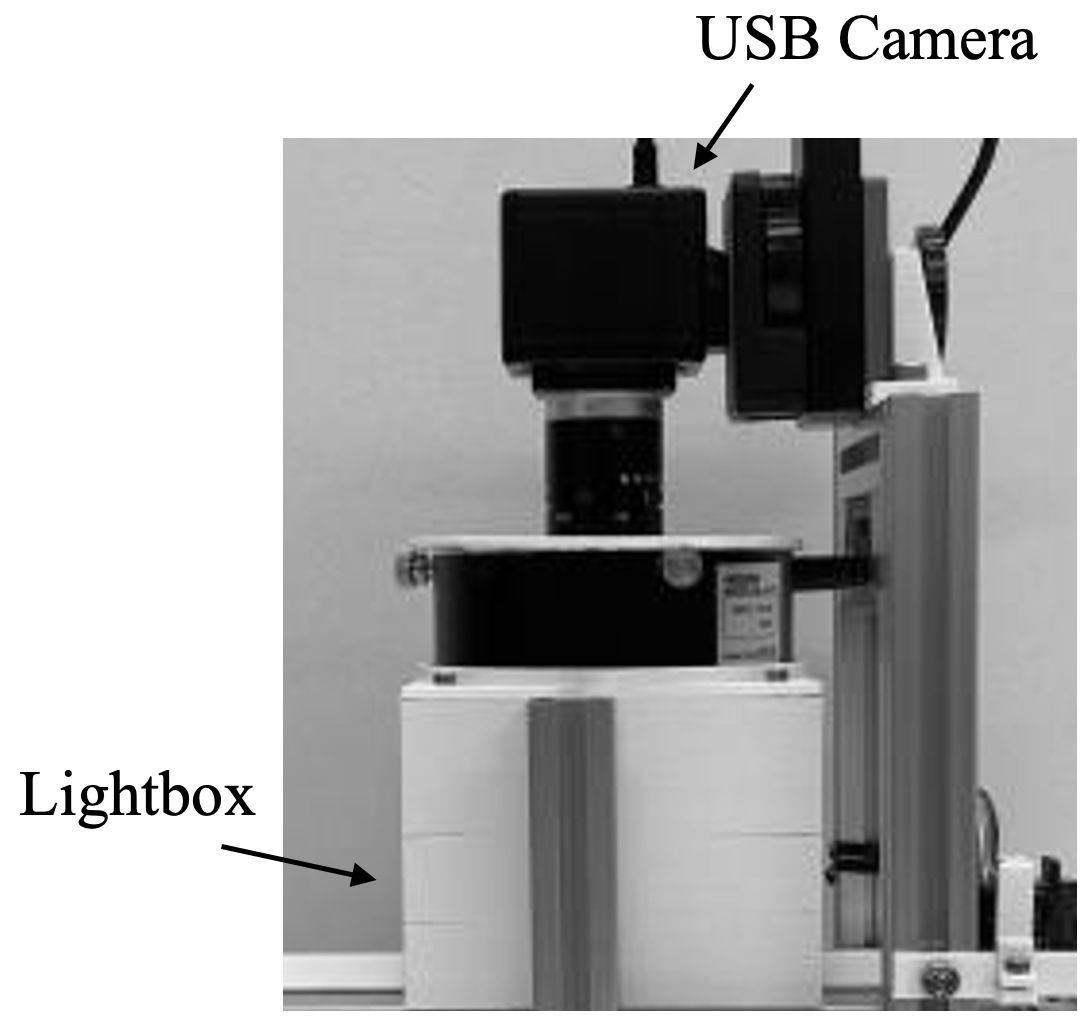
\includegraphics[scale = 0.5]{./chapter3/device.png}
    \caption{撮影環境}
    \label{fig_camera}
  \end{center}
\end{figure}

画像ごとに明度が変わったり影ができてしまうと誤判定の原因となってしまうため,Webカメラに自作のライトボックスを取り付けた.なお,本実験で使用したコーヒー豆はコロンビアスプレモとブラジルサントスNo.2の生豆である.図\ref{fig_beans}に実験環境で撮影した画像を示す.
\begin{figure}[htbp]
  \begin{center}
    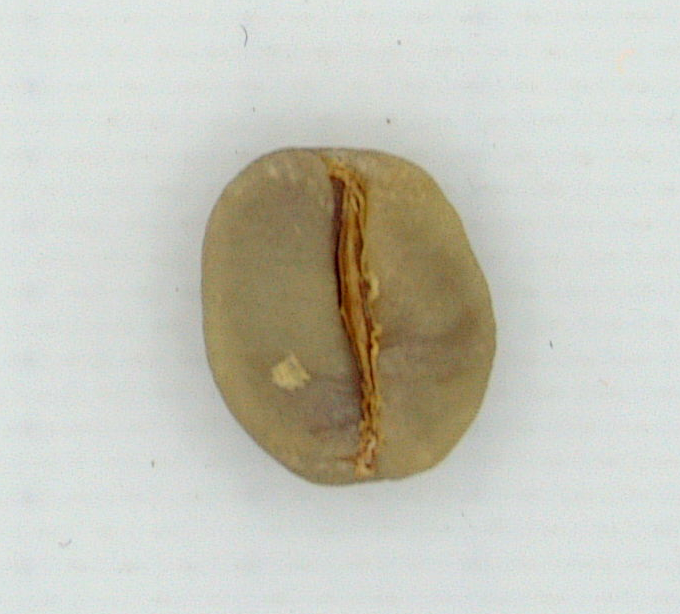
\includegraphics[scale = 0.35]{./chapter3/beans.png}
    \caption{撮影したコーヒー豆の画像}
    \label{fig_beans}
  \end{center}
\end{figure}

\subsection{画像の前処理}
取得画像には以下の前処理を施し,画像ごとの写り方をできるだけ統一した.
\begin{enumerate}
  \item ノイズ対策としてメディアンフィルタを用いたぼかし処理.
  \item 画像をグレースケール化し2値化をする.これによりコーヒー豆部分が黒く,背景が白い画像を生成する.
  \item 2値化した画像を反転し,コーヒー豆内のノイズを塗りつぶす.これによりコーヒー豆部分が白く,背景が黒い画像を生成する.
  \item その画像を元の画像と掛け合わせ,マスキングを行う.元の画像の背景のみ黒く塗りつぶす.
  \item コーヒー豆の重心を求め,$100\times 100$ピクセルに切り出す
  \item コーヒー豆を縦向きに補正
  \item 画像を$80\times 80$にリサイズし,コントラストを上げる.
\end{enumerate}

データセットの構成は以下の通りである.
\begin{itemize}
  \item 学習データ:3981枚
  \item テストデータ:789枚
\end{itemize}

\section{実験条件}
本実験のネットワークの構造を図\ref{fig_nnst}に示す.
\begin{figure}[htbp]
  \begin{center}
    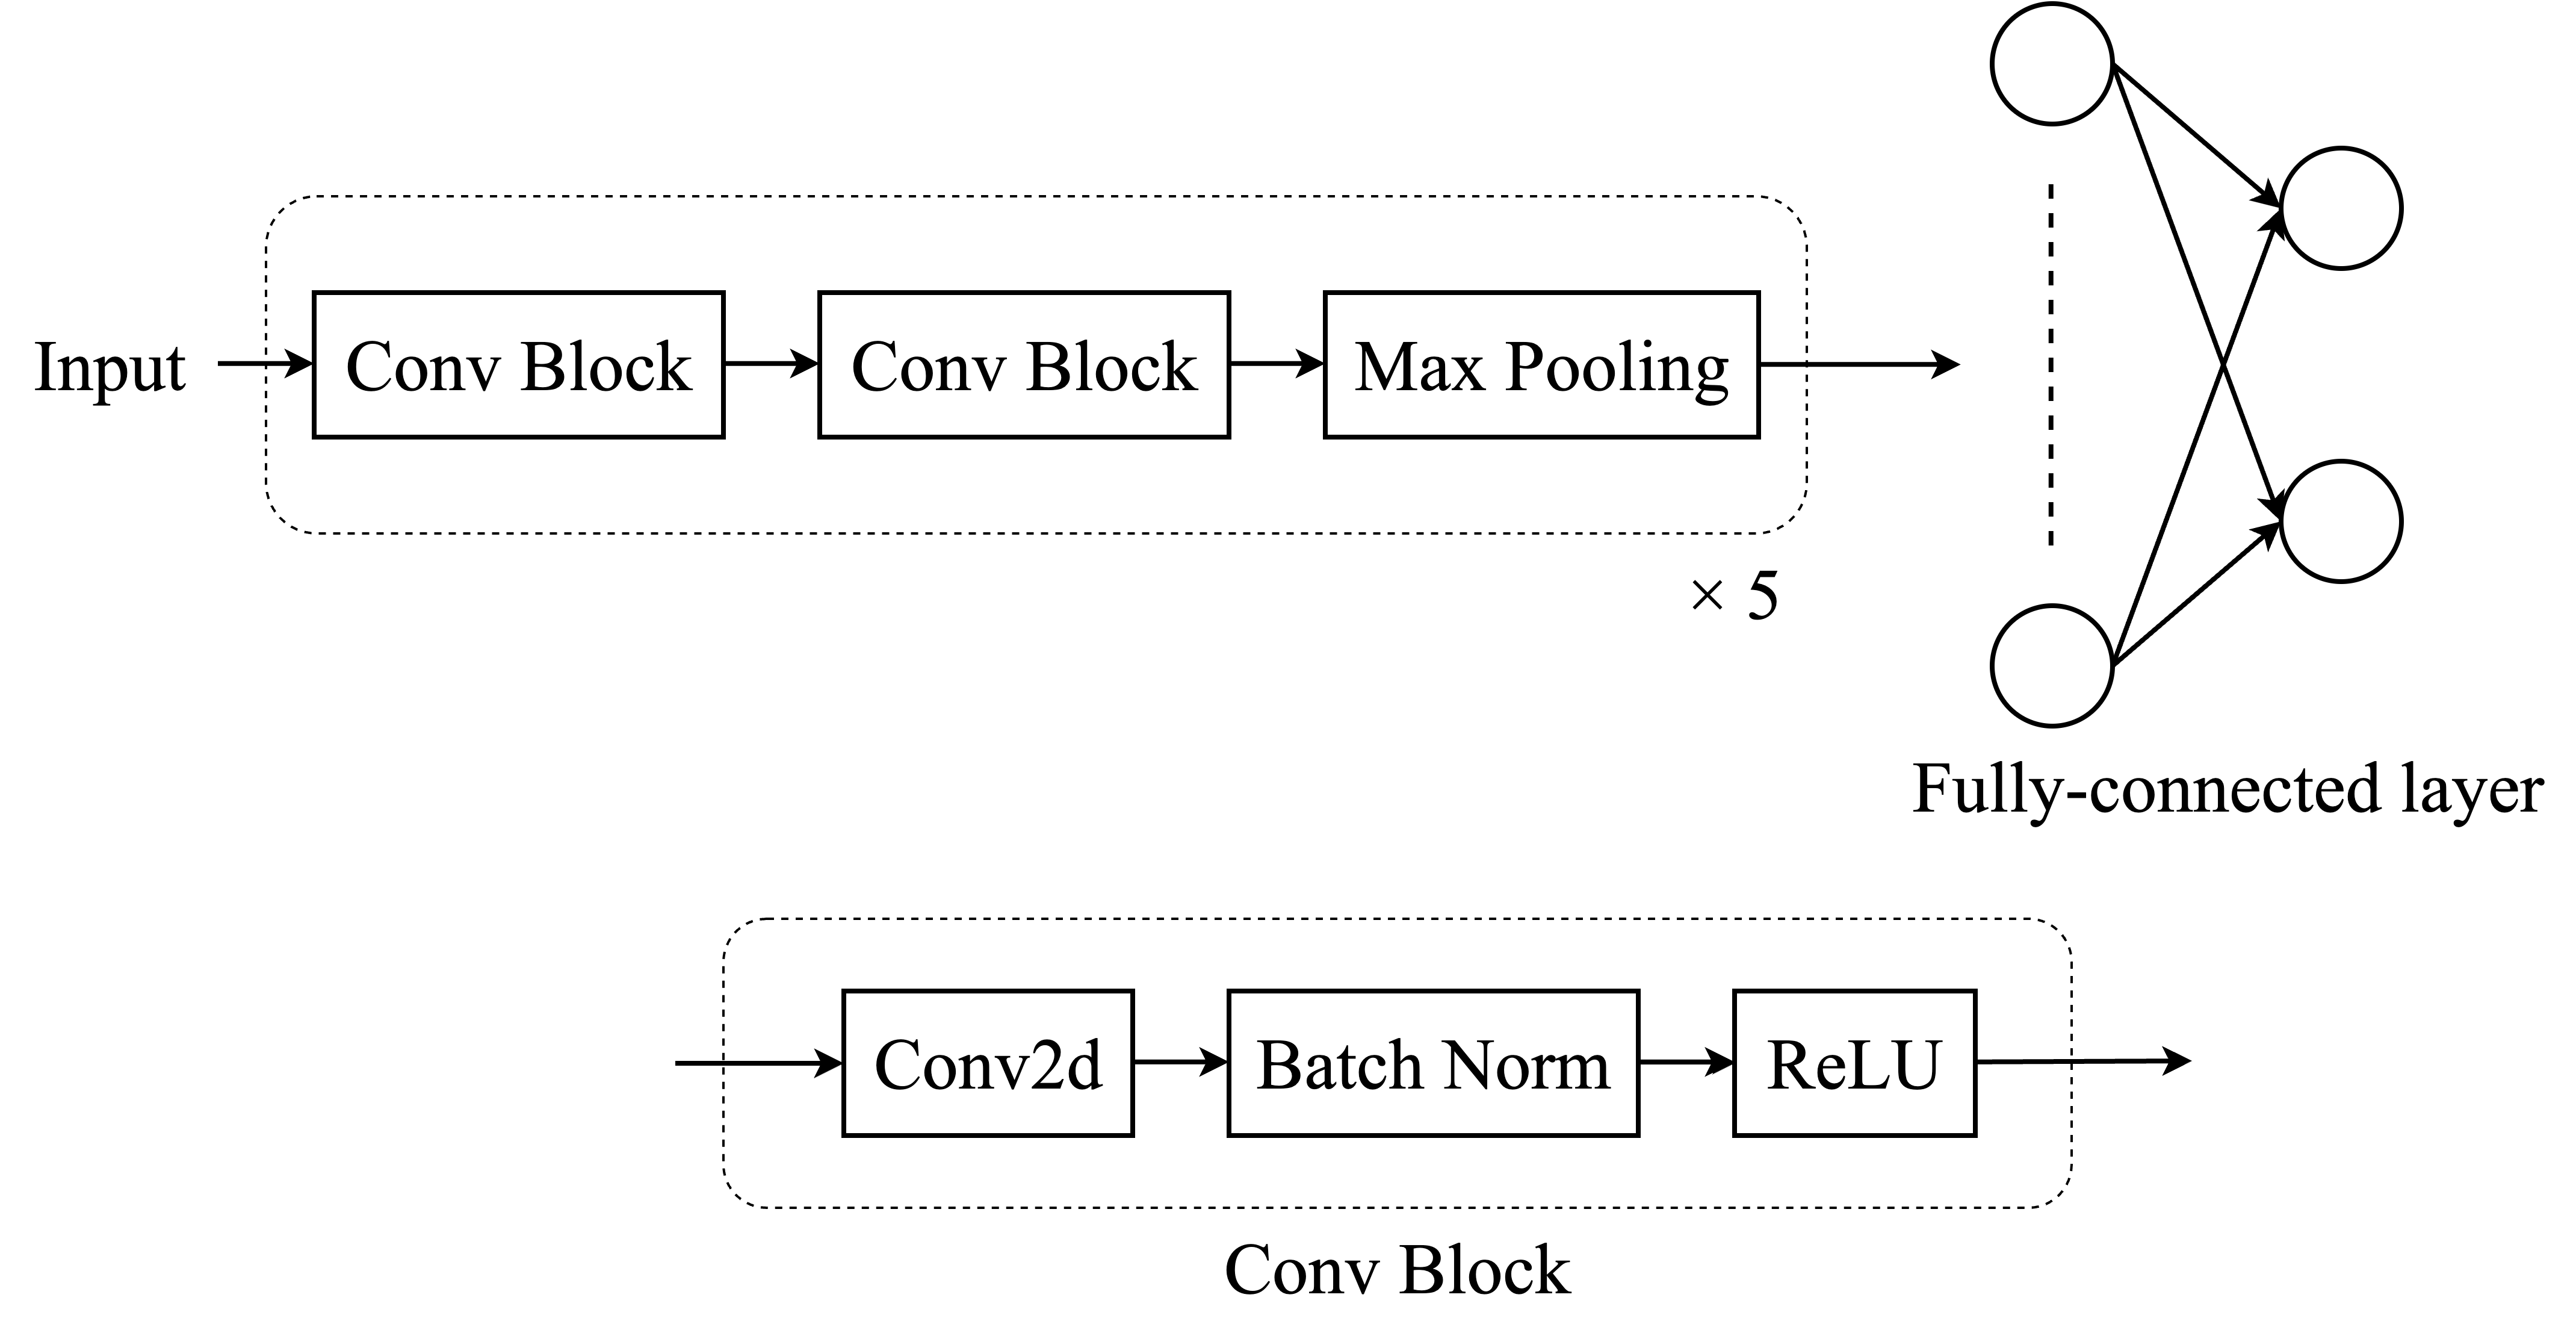
\includegraphics[scale = 0.08]{./chapter3/nn_struct.png}
    \caption{ネットワークの構造}
    \label{fig_nnst}
  \end{center}
\end{figure}

ネットワークの構造はVGG16\cite{simonyan2015deep}を参考に作成した.畳み込み,Batch Normalization,ReLUを1セットとして5回繰り返し合計で10層の畳み込み層とした.10層の畳み込み層を$C_1, C_2,  \ldots , C_{10}$として,各層のパラメータを表\ref{table_network_parameter}にまとめる.
\begin{table}
  \caption{ネットワークのパラメータ}
  \label{table_network_parameter}
  \centering
  \begin{tabular}{ccc}
    \hline
    畳み込み層  & カーネルサイズ & 出力ch \\
    \hline \hline
    $C_1$,$C_2$ & $3\times 3$ & 16\\
    $C_3$,$C_4$ & $3\times 3$ & 32\\
    $C_5$,$C_6$ & $3\times 3$ & 64\\
    $C_7$,$C_8$ & $3\times 3$ & 128\\
    $C_9$,$C_{10}$ & $3\times 3$ & 256\\
    \hline
    Max Pooling & カーネルサイズ$2\times 2$ & ストライド2\\
    全結合層 & 入力256 & 出力2\\
    \hline
  \end{tabular}
\end{table}
畳み込み層ではカーネルサイズはすべて$3\times 3$とし,出力のチャンネル数は畳み込み2層ごとに2倍している.1ピクセル分ゼロパディングを行っているため,畳み込み層では画像サイズを落としていない.Pooling層ではカーネルサイズ$2\times 2$,ストライド2のMax Poolingを行っており画像サイズを半分に落としている.そして,畳み込み層での結果にGrobal Avarage Poolingを行ったものを全結合層へ入力し,全結合層の出力は良否の2パターンになっている.
学習時はミニバッチ数32,エポック数400で学習を行っている.エポックごとに入力画像に対し
\begin{itemize}
  \item 水平方向の反転と回転
  \item 垂直方向の反転と回転
  \item 水平と垂直方向の反転と回転
  \item 回転のみ
\end{itemize}
を切り替えながらオンラインでデータの拡張を行った.誤差関数にはクロスエントロピー誤差を,最適化にはAdamを用いている.

BinaryConnectの検証時,ネットワークや学習時のパラメータはこのままに,以下の4つのネットワークを作成した.
\begin{itemize}
  \item CNN
  \item BinaryConnect
  \item BinaryConnect + Binarize Bias:バイアスも2値化したネットワーク
  \item BinaryConnect + None Bias:バイアスを消去したネットワーク
\end{itemize}
これら4種類のネットワークについて正答率や誤差の変化,学習の傾向などを検証しCNNの代替となるかを考察した.

\section{CNNとBinaryConnectの比較結果}
\subsection{判定精度の比較結果}
CNNとBinaryConnectの2つのネットワークについて判定精度と誤差のグラフを図\ref{fig_acc_loss_1}に示す.
これらの結果より,正答率やその推移はどちらのネットワークも同様の傾向を示していることが分かる.CNNの誤差は250Epoch近傍から上昇傾向にあるが,BinaryConnectでは200Epoch近傍まで減少傾向にあり,その後は維持をしている.このことから,CNNでは250Epoch以降過学習状態にあるが,BinaryConnectを用いることによって過学習を抑え学習できるようなモデルになっていると考えられる.
\begin{figure}[htbp]
  \begin{minipage}[b]{0.5\linewidth}
    \centering
    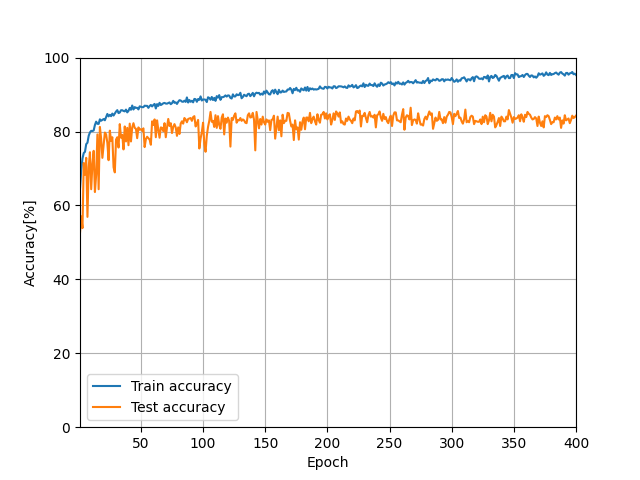
\includegraphics[keepaspectratio, scale=0.4]{./chapter4/acc_cnn.png}
    \subcaption{CNNでの正答率の推移}
  \end{minipage}
  \begin{minipage}[b]{0.5\linewidth}
    \centering
    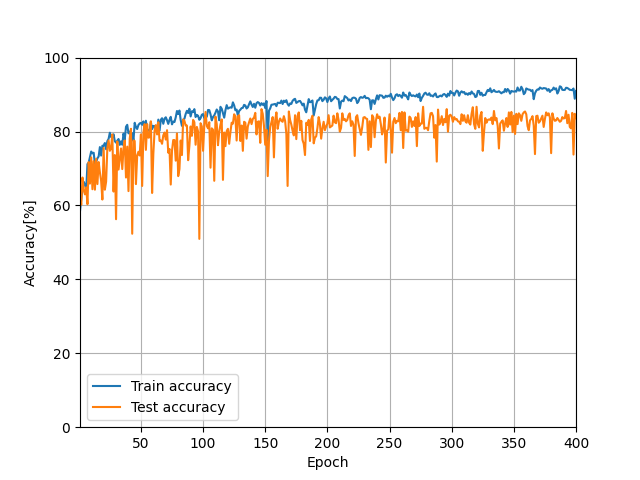
\includegraphics[keepaspectratio, scale=0.4]{./chapter4/acc_bc.png}
    \subcaption{BinaryConnectによる正答率の推移}
    \label{fig_acc_bc}
  \end{minipage}\\
  \begin{minipage}[b]{0.5\linewidth}
    \centering
    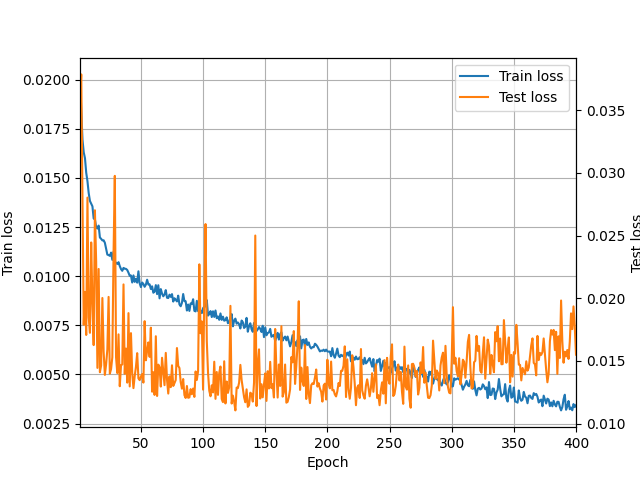
\includegraphics[keepaspectratio, scale=0.4]{./chapter4/loss_cnn.png}
    \subcaption{CNNでの誤差の推移}
  \end{minipage}
  \begin{minipage}[b]{0.5\linewidth}
    \centering
    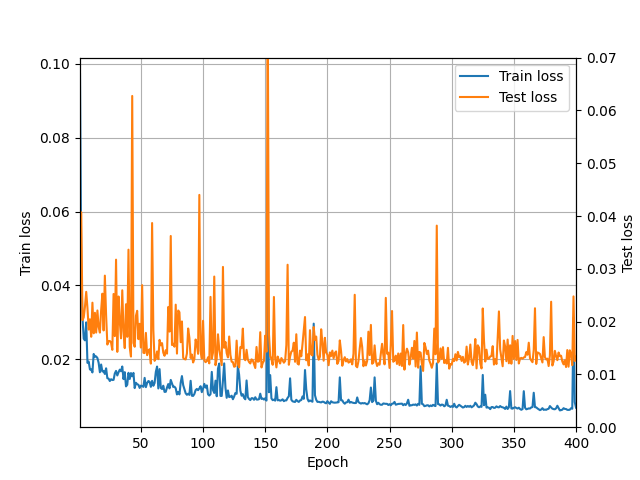
\includegraphics[keepaspectratio, scale=0.4]{./chapter4/loss_bc.png}
    \subcaption{BinaryConnectによる誤差の推移}
  \end{minipage}
  \caption{CNNとBinaryConnectによる学習結果}
  \label{fig_acc_loss_1}
\end{figure}

また,CNNに比べBinaryConncetでは判定精度にばらつきがありLossの値も大きくなっていることが分かる.各ネットワークの最終10Epochの平均正答率をまとめると以下のようになった.
\begin{itemize}
  \item CNN:83.57\%
  \item BinaryConnect:82.53\%
  % \item BinaryConnect(Binarize Bias):82.30\%
  % \item BinaryConnect(No Bias):82.50\%
\end{itemize}

この結果から分かる通り,BinaryConnectでは正答率にばらつきがあるが,正答率に大きな差はない.今回のネットワークの構造において,1178288個の重みがあり,32bitの浮動小数で表されるCNNでは重みだけで約4.7MBのメモリを消費する.しかしBinaryConnectを使用することで重みは約117KBまで削減することができる.ここまでの情報量を削減して同等の正答率を確保できることは,BinaryConnectが計算リソースの削減に有効であるといえる.

\section{BinaryConnectの重みの推移}
BinaryConnectの正答率はEpochごとのばらつきが大きくなっている.これは0付近で揺れている重みを強制的に2値化するためフィルタが大きく変化することによるものではないかと考えた.図\ref{fig_acc_bc}の実験結果で,378Epoch目の正答率は約84.92\%,379Epoch目の正答率は83.77\%,380Epoch目の正答率は74.14\%である.378Epochと379Epochでは正答率がほぼ同じだが,379Epochと380Epochでは約10ポイント低下している.そこで各Epochにおける層ごとの-1の個数の変化率を検証した.その結果を表\ref{table_parameter_transition}にまとめる.
\begin{table}
  \caption{Epochごとの重みの変化率}
  \label{table_parameter_transition}
  \centering
  \begin{tabular}{ccc}
    \hline
    Layer & 378$\to$379Epoch(\%) & 379$\to$380Epoch(\%) \\
    \hline \hline
    $C_1$ & 0.833 & 2.439\\
    $C_2$ & 0.476 & 0.395\\
    $C_3$ & 1.244 & 0.256\\
    $C_4$ & 0.061 & 0.492\\
    $C_5$ & 0.030 & 0.070\\
    $C_6$ & 0.344 & 0.257\\
    $C_7$ & 0.226 & 0.002\\
    $C_8$ & 0.094 & 0.058\\
    $C_9$ & 0.013 & 0.117\\
    $C_{10}$ & 0.099 & 0.092\\
    全結合層 & 0 & 1.090\\
    \hline
  \end{tabular}
\end{table}

この結果をみると正答率が変わらないときに比べ,減少する時は入力層,出力層においての-1の変化率が大きくなっていることが分かる.隠れ層では両者に大きな差はないことから,重みの正答率への影響は入口や出口で顕著に現れると考えられる.重みのばらつきを抑え正答率を上げるためにはネットワークの入出力付近の重みや勾配をクリッピングしたり,-1と1の他に0を重みに追加した3値化\cite{li2022ternary}を行うなどの対策が考えられる.

\subsection{混同行列および不正解画像}
CNNとBinaryConnectにおいて,推論の傾向を混同行列として表\ref{table_conf}に示す.数字は左側がCNN,右側がBinaryConnectの結果である.
\begin{table}[htbp]
  \caption{最終Epoch時の推論と正解の結果}
  \label{table_conf}
  \centering
  \begin{tabular}{cc|cc}
    \multicolumn{2}{c|}{} & \multicolumn{2}{c}{推論}\\
    &  & 正常豆& 欠点豆\\
    \hline
    \multirow{2}{*}{正解}& 正常豆& 332, 369& 58, 100\\
    & 欠点豆& 66, 29& 333, 291
  \end{tabular}
\end{table}

この結果から,CNNは正常豆も欠点豆も満遍なく判別するが,BinaryConnectでは正常豆を欠点豆と判断してしまうケースが多くあることがわかった.品質のことのみを考えると欠点豆が混入しにくいため高品質な生豆を選別することができる.一方,一般家庭での使用を考えると正常豆を大量に捨てることになるため改善の必要がある.

また,最終的に推論が不正解になった画像を確認すると,人間が見ても判別しにくいものが誤判定される傾向にあった.不正解になった画像を図\ref{fig_false_image}に示す.
特にチャフと呼ばれる茶色の薄皮が張り付いているものや形状的に影ができてしまうものは不正解が多かった.これは欠けがあるように誤判定されているのではと考えられる.また,小さい豆を判別することが難しく,これは学習による判別ではなく面積による判別を行うなど検討が必要である.しかし,カビ豆や虫食い豆などの重度の欠点豆は取り除くことができており,食品衛生的な観点から見ると良い選別結果であると言える.これはCNN,BinaryConnectともに同様な傾向を示していた.
\begin{figure}[htbp]
  \begin{minipage}[b]{0.5\linewidth}
    \centering
    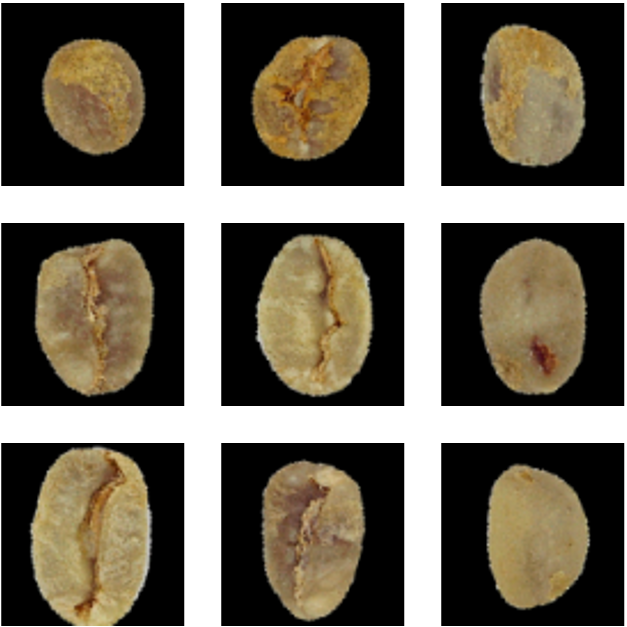
\includegraphics[keepaspectratio, scale=1]{./chapter4/false_normal.png}
    \subcaption{正常豆}
  \end{minipage}
  \begin{minipage}[b]{0.5\linewidth}
    \centering
    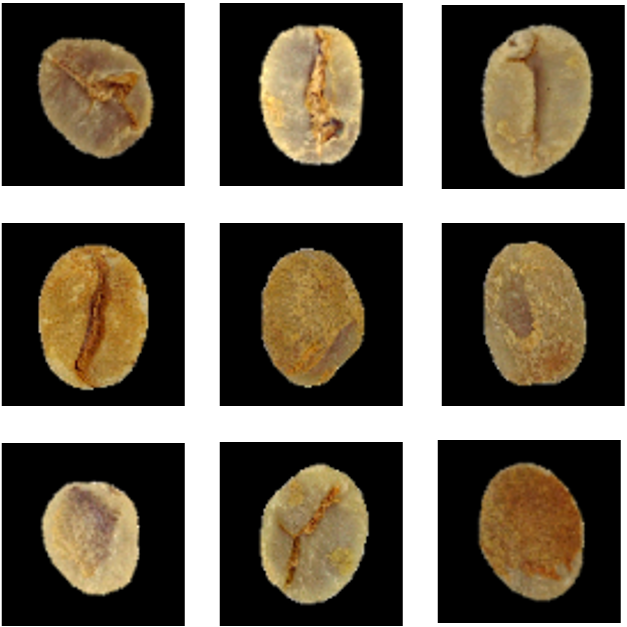
\includegraphics[keepaspectratio, scale=1]{./chapter4/false_anomaly.png}
    \subcaption{欠点豆}
  \end{minipage}
  \caption{推論の結果が不正解になった画像}
  \label{fig_false_image}
\end{figure}

\section{バイアスによる判定精度の違い}
計算リソースの削減として,普通32ビットの浮動小数で表されるバイアスを2値化もしくは消去した際の判定精度を通常のBinaryConnectと比較する.BinaryConnectのバイアスを2値化した時と消去した時の正答率と誤差を図\ref{fig_acc_loss_2}に示す.
\begin{figure}[htbp]
  \begin{minipage}[b]{0.5\linewidth}
    \centering
    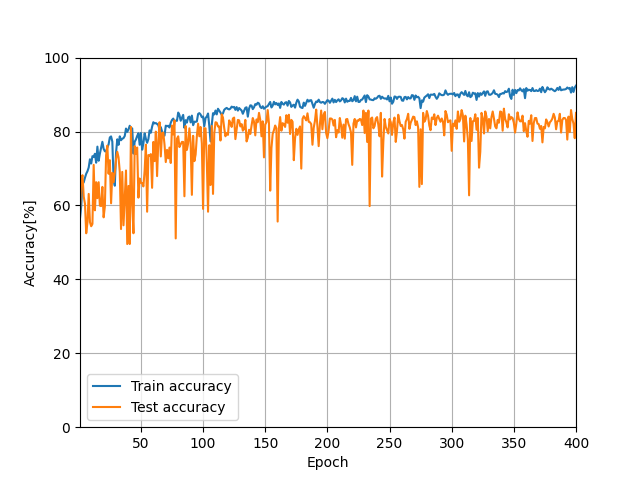
\includegraphics[keepaspectratio, scale=0.4]{./chapter4/acc_bwb.png}
    \subcaption{BinaryConnect+バイアスの2値化での正答率の推移}
  \end{minipage}
  \begin{minipage}[b]{0.5\linewidth}
    \centering
    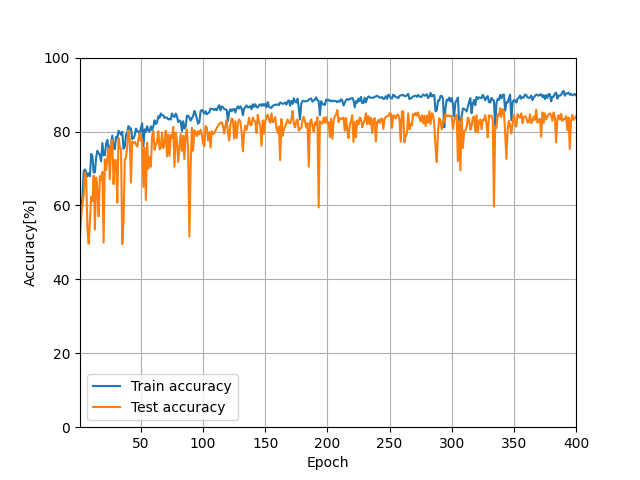
\includegraphics[keepaspectratio, scale=0.4]{./chapter4/acc_bc_nb.png}
    \subcaption{BinaryConnect+バイアスの消去による正答率の推移}
  \end{minipage}\\
  \begin{minipage}[b]{0.5\linewidth}
    \centering
    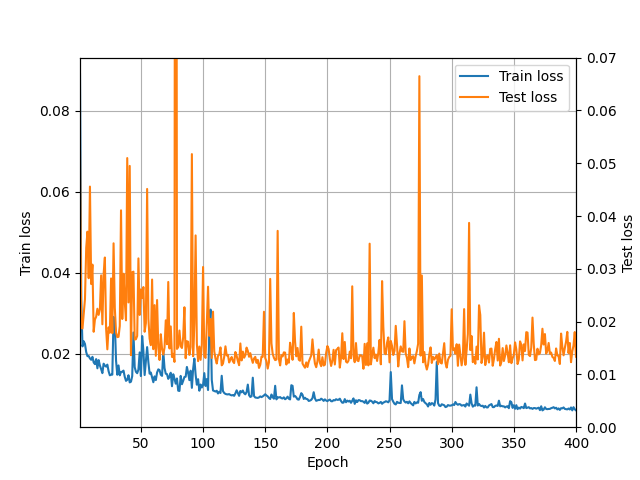
\includegraphics[keepaspectratio, scale=0.4]{./chapter4/loss_bwb.png}
    \subcaption{BinaryConnect+バイアスの2値化での誤差の推移}
  \end{minipage}
  \begin{minipage}[b]{0.5\linewidth}
    \centering
    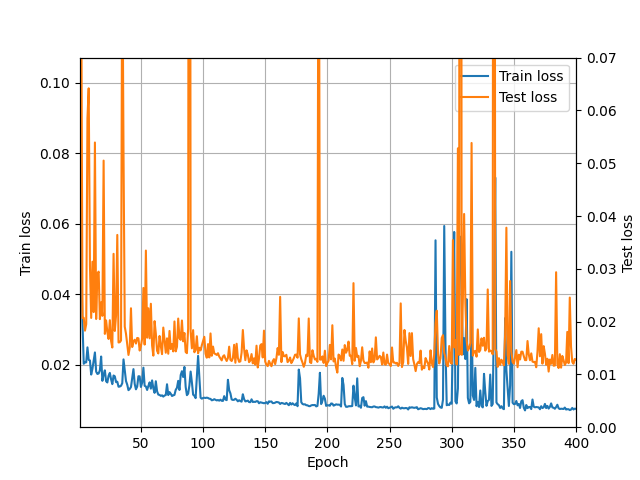
\includegraphics[keepaspectratio, scale=0.4]{./chapter4/loss_bc_nb.png}
    \subcaption{BinaryConnect+バイアスの消去による誤差の推移}
  \end{minipage}
  \caption{BinaryConnectのバイアスを2値化,消去させた学習結果}
  \label{fig_acc_loss_2}
\end{figure}

各ネットワークの最終10Epochの平均正答率は以下のようだった.
\begin{itemize}
  \item BinaryConnect(Binarize Bias):82.30\%
  \item BinaryConnect(None Bias):82.50\%
\end{itemize}
BinaryConnectのみの平均正答率が82.53\%であったことを考えると,バイアスを2値化,消去しても正答率への影響は少ないことが分かる.バイアスは重みほど計算リソースを圧迫しないが,32bitの浮動小数を持ち,深層化するとメモリの消費量も無視できない.バイアスを消去しても同等の性能を示すことはこの手法も計算コストの削減として有効であるといえる.
